\documentclass[11pt]{article}
\usepackage{amssymb,amsmath}
\usepackage{color,soul}
\usepackage{tikz,ifthen,calc}
\usetikzlibrary{positioning}
\usetikzlibrary{shapes}
\usetikzlibrary{shapes.symbols,patterns}
\usetikzlibrary{calc,through,backgrounds}
\usetikzlibrary{decorations.pathreplacing}
\usetikzlibrary{shapes.geometric, arrows}

\begin{document}

	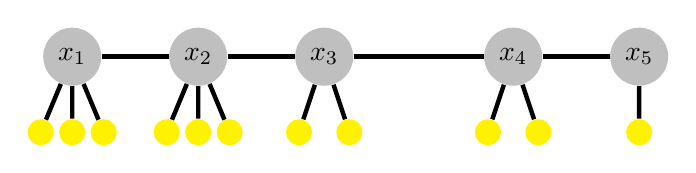
\begin{tikzpicture}[scale=0.8]

		\def\pathlen{5}
		\def\pathspacing{2.3}
		\pgfmathtruncatemacro{\plenplusone}{\pathlen + 1}

		\foreach \x in {1,...,\pathlen} {
		\pgfmathtruncatemacro{\xcoord}{\x * \pathspacing}
		\node [minimum size= 3mm,fill=lightgray,circle] (v\x) at (\xcoord,0)  {$x_{\x}$};
		}

	\pgfmathtruncatemacro{\xcoord}{1 * \pathspacing}				\node [fill=yellow,circle] (leaf1) at ( \xcoord - .5, - 1.2)  {};
	\path [draw=black,ultra thick] (leaf1) [-] edge (v1);

	\node [fill=yellow,circle] (leaf2) at ( \xcoord, - 1.2)  {};
	\path [draw=black,ultra thick] (leaf2) [-] edge (v1);

	\node [fill=yellow,circle] (leaf3) at ( \xcoord + .5, - 1.2)  {};
	\path [draw=black,ultra thick] (leaf3) [-] edge (v1);

	\pgfmathtruncatemacro{\xcoord}{2 * \pathspacing}					
	\node [fill=yellow,circle] (leaf1) at ( \xcoord - .5, - 1.2)  {};
	\path [draw=black,ultra thick] (leaf1) [-] edge (v2);

	\node [fill=yellow,circle] (leaf2) at ( \xcoord, - 1.2)  {};
	\path [draw=black,ultra thick] (leaf2) [-] edge (v2);

	\node [fill=yellow,circle] (leaf3) at ( \xcoord + .5, - 1.2)  {};
	\path [draw=black,ultra thick] (leaf3) [-] edge (v2);		

	\pgfmathtruncatemacro{\xcoord}{3 * \pathspacing}

	\node [fill=yellow,circle] (leaf1) at ( \xcoord - .4, - 1.2)  {};
	\path [draw=black,ultra thick] (leaf1) [-] edge (v3);

	\node [fill=yellow,circle] (leaf3) at ( \xcoord + .4, - 1.2)  {};
	\path [draw=black,ultra thick] (leaf3) [-] edge (v3);		

	\pgfmathtruncatemacro{\xcoord}{4 * \pathspacing}				
	\node [fill=yellow,circle] (leaf1) at ( \xcoord - .4, - 1.2)  {};
	\path [draw=black,ultra thick] (leaf1) [-] edge (v4);

	\node [fill=yellow,circle] (leaf3) at ( \xcoord + .4, - 1.2)  {};
	\path [draw=black,ultra thick] (leaf3) [-] edge (v4);		

	\pgfmathtruncatemacro{\xcoord}{5 * \pathspacing}					
	\node [fill=yellow,circle] (leaf1) at ( \xcoord, - 1.2)  {};
	\path [draw=black,ultra thick] (leaf1) [-] edge (v5);

	\pgfmathtruncatemacro{\plenminusone}{\pathlen - 1}
	\foreach \x in {1,...,\plenminusone}{

		\pgfmathtruncatemacro{\xpp}{\x+1}
		\path [draw=black,ultra thick] (v\x) edge (v\xpp);

	}
\end{tikzpicture}

\end{document}